\subsection{Terrain Generation}

The terrain generator constructs the landscape on which the city can be assembled upon.
It generates a mesh congregated out of triangles and a perlin noise generator to apply height to the triangles' connection points.
Naturally, other generators need to take into account the height of the terrain and avoid uninhabitable areas like water and very steep hills.
The mesh is then textured by applying one texture to the terrain.
The texture’s colour will evanesce between other colours depending on the height level of the terrain (and water) to illustrate the ground type at the current height level.f

The city could have been generated on a flat plane, which does have its advantages since more time could be spent on creating the city.
However, a city surrounded by a landscape would result in a more realistic and vivid setting, which would indirectly make the city look better.
A plane that could simulate a basic, yet somewhat realistic, environment for the city to be generated upon was a self-evident feature that would be included in the project.
The generated environment would be decided to be referred to as terrain.
This terrain would be based on real-world aesthetics and therefore include natural biomes such as such as snowy mountains, grassland, hills and bodies of water (specifically oceans/lakes).
Additional aspects would bypass the range of the project’s goals since the core focus of this project was the city, not the terrain.
Therefore, a decision was made to keep the terrain looking rather primitive, i.e. that it would be limited and expected to include: 

\begin{easylist}
 @ A 2D plane to represent the ground.
 @ The plane’s shape, as in bumps, hills and valleys.
 @ Another 2D plane to represent water.
 @ Textured water and ground depending on height of a certain point of the plane.
\end{easylist}

The terrain base could have been created in two ways: either using a custom mesh made of triangles or using an advanced, built-in terrain mesh API provided by Unity.
Both options had their advantages and disadvantages.
Utilizing meshes means that the ground is created by connecting triangles to one another in a pattern.
However height-based texture splatting could be problematic for the reason that a custom shader would have to be created that performs the blending of textures.
This would lead to issues when exporting the terrain, along with the fact that more programming has to be done for this task.
On the other hand, the API is easy to fabricate and manipulate along with extensive documentation to encompass its functionalities.
For instance, texture splatting is incorporated to the API, which would make the process of generating textures much simpler.

In the first iteration for the terrain base, the API by Unity seemed reasonable as primary choice because of its simplicity and availability.
Unfortunately, the API did not produce traditional meshes, and instead produced dynamically adapting objects specific to Unity.
To export such a terrain, one would have to first convert it into a traditional mesh.
Converting the mesh was done easily using Unity Editor packages, however those tools would be inaccessible when compiling the final application.
Including Unity’s packages’ tools to convert the terrain object was not a trivial task.
Because of this, the API had to be scrapped and the terrain was instead generated using the alternative option.
To counteract the need to program a custom shader, the terrain only contained one texture which was gradually saturated with a different colour to illustrate the expected type of ground existing on that height level.
Specifically, the texture’s colour would be shifted toward a white colour to illustrate mountain tops, a brown colour for hills, green for low ground grassland and a beige-yellow colour for heights slightly above water.
Water is unaffected by this.

The next decision was to pick an algorithm that could designate height levels for the flat plane, i.e. to shape it with inward and outward facing dents that would represent valleys/ocean and mountains respectively.
It was decided that the terrain was to be procedurally generated, as it would allow drastically more varied content in the generator.
The most common algorithms considered that could solve this task were simplex noise and perlin noise.
The noise functions work by creating vectors which randomizes the influx of vectors to specific points.
The vectors’ directions determined whether or not the point (in our case) should be raised or lowered on the plane.
\begin{figure}[h!]
  \centering

  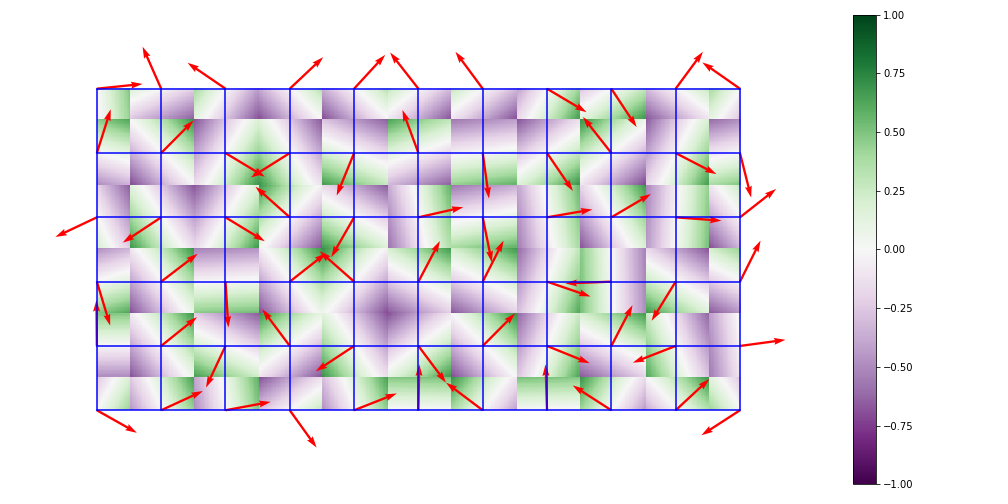
\includegraphics[width=0.8\textwidth]{figure/perlin_noise_gradient_grid.png}
  \caption{Grid of vectors that determine the values for each point on the plane. \cite{noise_grid_img}. Vectors pointing towards points increases their value, whilist vectors pointing away from points leaves them with decreased value.}

  \label{fig:noise_grid}
\end{figure}
The output from these functions would be the exact height value, which would shape the terrain in a smooth manner similar to real-world landscape.
The differences between simplex noise and perlin noise are small, but in short, simplex noise computes calculations more efficiently than perlin noise \cite{simplexnoise_stefan}.
The noise values were in the end collected from the noise generator module, which was based on simplex noise.

The final aspect to include in the terrain was texture.
A blank, white canvas would not be appropriate as an environment, as it would appear glaringly unrealistic.
Therefore textures were implemented to grant the terrain the appearances of grass, mountains, water etc. to showcase their existence.
These following bullet points are what was expected of the textures:

\begin{easylist}
 @ Oceans and lakes should have a blue tint.
 @ Terrain slanting towards oceans with low steepness should transition into beaches.
 @ Spacious plains should cover various shades of green.
 @ Mountains should appear rocky.
 @ Tall mountain peaks should be covered in snow.
\end{easylist}


The textures were taken from Unity’s asset store community, along with the Standard Assets made by Unity themselves.
After a lot of searching, the most effortless choice for the water texture was taken from Standard Assets by Unity.
The rest of the textures were borrowed and resized from Aleksey Pakhalchyk's work (a.k.a. ``ALP8310''  on Unity Asset Store) \cite{ALP8310}.
For the grass, mountain, snow and sand, they all had the same texture as explained previously.
